% Define document class
\documentclass{aastex631}
% \usepackage{showyourwork}
\usepackage{float}
\usepackage{amsmath}
\usepackage{amssymb}
\usepackage{hyperref}
\usepackage{bm}
\usepackage{listings}


\newcommand\twostep{two-step\xspace}
\newcommand\full{full-fledged\xspace}

\DeclareMathOperator*{\argmax}{arg\,max}
\DeclareMathOperator*{\argmin}{arg\,min}
\newcommand{\set}[1]{\{\,#1\,\}}
\newcommand{\nuance}{\texttt{nuance}}
\newcommand{\TODO}{\textcolor{red}{TODO}}

\lstdefinestyle{mystyle}{
    backgroundcolor=\color{gray!5},
    commentstyle=\color{gray!70},
    keywordstyle=\color{Bittersweet},
    stringstyle=\color{RoyalBlue},
    basicstyle=\fontsize{7.5}{11}\fontfamily{DejaVuSansMono-TLF}\selectfont,
    breakatwhitespace=false,         
    breaklines=true,
    rulecolor=\color{black!15},
    numbers=left,
    numberstyle=\fontsize{7}{11}\fontfamily{DejaVuSansMono-TLF}\selectfont\color{gray!50},
    framerule=0pt,
    breakindent=0pt,
    resetmargins=true,
    numbersep=5pt,
    frame=single,
    aboveskip=1em,
    belowskip=1em,
}
\lstset{style=mystyle}

% Cortex style
% All the packages
\usepackage{url}
\usepackage{amsmath}
\usepackage{mathtools}
\usepackage{amssymb}
\usepackage{natbib}
\usepackage{graphicx}
\usepackage{calc}
\usepackage{etoolbox}
\usepackage{xspace}
\usepackage[T1]{fontenc} % https://tex.stackexchange.com/a/166791
\usepackage{textcomp}
\usepackage{ifxetex}
\ifxetex
\usepackage{fontspec}
\defaultfontfeatures{Extension = .otf}
\fi
\usepackage{fontawesome}
\usepackage{listings}


% Here goes the github repo
% \newcommand{\githublink}{https://github.com/lgrcia/paper-nuance/tree/main}
\newcommand{\codelink}[1]{\href{githublink#1.py}{\codeicon}\,\,}
\newcommand{\animlink}[1]{\href{githublink#1.gif}{\animicon}\,\,}
\newcommand{\prooflink}[1]{\href{\githublink/proofs/#1.ipynb}{\raisebox{-0.1em}{\prooficon}}}


% Shorthand for this paper
\newcommand{\Python}{\textsf{Python}\xspace}
\newcommand{\cpp}{\textsf{C}++\xspace}

% References to text content
\newcommand{\documentname}{\textsl{article}}
\newcommand{\figureref}[1]{\ref{fig:#1}}
\newcommand{\Figure}[1]{Figure~\figureref{#1}}
\newcommand{\figurelabel}[1]{\label{fig:#1}}
\renewcommand{\eqref}[1]{\ref{eq:#1}}
\newcommand{\Eq}[1]{Equation~(\eqref{#1})}
\newcommand{\eq}[1]{\Eq{#1}}
\newcommand{\eqalt}[1]{Equation~\eqref{#1}}

% Add code, proof, and animation hyperlinks
\definecolor{linkcolor}{rgb}{0.1216,0.4667,0.7059}
\newcommand{\codeicon}{{\color{linkcolor}\faFileCodeO}}
\newcommand{\prooficon}{{\color{linkcolor}\faPencilSquareO}}
\newcommand{\githublink}{https://github.com/lgrcia/paper-nuance/tree/main}
\newcommand{\codelink}[1]{\href{githublink#1.py}{\codeicon}\,\,}
\newcommand{\animlink}[1]{\href{githublink#1.gif}{\animicon}\,\,}
\newcommand{\prooflink}[1]{\href{\githublink/proofs/#1.ipynb}{\raisebox{-0.1em}{\prooficon}}}


% Define a proof environment for open source equation proofs
\newtagform{eqtag}[]{(}{)}
\newcommand{\currentlabel}{None}
\newenvironment{proof}[1]{%
\ifstrempty{#1}{%
\renewtagform{eqtag}[]{\raisebox{-0.1em}{{\color{red}\faPencilSquareO}}\,(}{)}%
}{%
\renewtagform{eqtag}[]{\prooflink{#1}\,(}{)}%
}%
\usetagform{eqtag}%
\renewcommand{\currentlabel}{#1}
\align%
}{%
\endalign%
\renewtagform{eqtag}[]{(}{)}%
\usetagform{eqtag}%
\message{<<<\currentlabel: \theequation>>>}%
}

% Define the `oscaption` command for open source figure captions
\newcommand{\oscaption}[2]{\caption{#2 \codelink{#1}}}

% Code examples
\definecolor{codegreen}{rgb}{0,0.6,0}
\definecolor{codegray}{rgb}{0.5,0.5,0.5}
\definecolor{codepurple}{rgb}{0.58,0,0.82}
\definecolor{backcolour}{rgb}{0.95,0.95,0.95}
\lstdefinestyle{mystyle}{
    backgroundcolor=\color{backcolour},
    commentstyle=\color{codegreen},
    keywordstyle=\color{magenta},
    numberstyle=\tiny\color{codegray},
    stringstyle=\color{codepurple},
    basicstyle=\small\ttfamily,
    breakatwhitespace=false,
    breaklines=true,
    captionpos=b,
    keepspaces=true,
    numbers=left,
    numbersep=5pt,
    showspaces=false,
    showstringspaces=false,
    showtabs=false,
    tabsize=2,
    aboveskip=1em,
    belowskip=1em,
    keywords=[2]{map},
    keywordstyle=[2]{\color{black!80!black}},
    upquote=true
}
\lstset{style=mystyle}

% Typography obsessions
\setlength{\parindent}{3.0ex}
\renewcommand\quad{\hskip\fontdimen3\font}


% Begin!
\begin{document}

% Title
\title{\texttt{nuance}: Detection of planetary transits in the presence of correlated noise}

% Authors list
\author{Lionel J. Garcia}
\affiliation{Astrobiology Research Unit, Universit\'{e} de Li\`{e}ge, All\'{e}e du 6 Ao\^{u}t 19C, B-4000 Li\`{e}ge, Belgium}
\author{Daniel Foreman-Mackey}
\affiliation{Center for Computational Astrophysics, Flatiron Institute, New York, NY, USA}
\author{Francisco J. Pozuelos}

\correspondingauthor{Lionel J. Garcia}
\email{lionel\_garcia@live.fr}

% Abstract with filler text
\begin{abstract}
    We present \nuance{}, an algorithm to search for planetary transits in light curves featuring correlated noise, such as instrumental signals and stellar photometric variability. To deal with these nuisance signals, a common approach consists in cleaning a light curve from correlated noise before searching for transits. However, we show that this approach, based on the prior assumption that transits are not present, strongly degrades their signals, up to the point of no detection. As this degradation depends on the correlated noise characteristics, we explore the parameter space for which transits are altered, and quantify this effect on a wide variety of cases. We show that \nuance{} outperforms the detection capabilities of commonly used transit search algorithms, especially for light curves featuring correlated noise with an amplitude three times greater than the searched transit depth. We perform our tests by injecting transits on synthetic light curves, and on known TESS candidates light curves to assess the performance of our algorithm on realistic multi-planetary systems datasets. Beyond its detection efficiency, we make \nuance{} tractable, \TODO{} times faster than current alternatives based on brute force detrending, and available as a well documented open-source Python package\footnote{\href{https://github.com/lgrcia/nuance}{https://github.com/lgrcia/nuance}}.
\end{abstract}

% Main body with filler text
\section*{Introduction}
\label{sec:intro}
Exoplanets, planets outside our solar system, are discovered at an ever-increasing rate. Beyond the study of their inner structure and atmosphere, they give a unique glimpse to extrasolar systems' formation, dynamics, as well as being probes to understand exoplanets' host stars. This is particularly true for systems whose orbital plane is aligned with our line of sight, leading to observable planetary transits. Although these transit signals can be seen in the apparent flux received from their stars, they are often mixed with other astrophysical and instrumental signals. 
If they can be disentangled from these nuisance signals, transits offer a powerful way to detect exoplanets. However, disentangling these signals comes with many challenges. Due to their nature we will refer to these nuisance signals as correlated noise.
\\\\
Widely used transit-search algorithms (\cite{bls}) are capable of detecting transits on light curves containing only transits and white noise. Hence, the simplest way to find periodic transit signals is to first clean a light curve from nuisance signals before performing the search. This strategy is widely adopted by the community, both using physically-motivated systematics models like \cite{everest1, everest2}, or empirical filtering techniques, such as the ones described and implemented in \cite{wotan}. However, when correlated noise start resembling transits, this cleaning step (often referred to as \textit{detrending}) is believed to degrade their detectability. In this case, the only alternative to search for transits is to perform a full-fledged modeling of the light curve, including both transits and correlated noise, and asses the likelihood of the data to the transit model on a wide parameter space, an approach largely avoided due to its intractable nature. Nonetheless, \citealt{kovacs2016} ask: \textit{Periodic transit and variability search with simultaneous systematics filtering: Is it worth it?}, and answer \textit{no}. Although the latter study discards the benefit of using a full-fledged approach in the general case, it fails at exploring the light-curves characteristics for which it becomes necessary.\\

% While it might only represent a handful of systems, this cases are extremely valuable for the exoplanetary science community. First, variability may be associated with star-spots that can be probed with the help of planetary transits. A better understanding of these structures benefit both the study of stellar atmospheres and their concerning impact on planetary atmosphere retrievals. Second, the growing interest of the community for ultra-cool dwarf stars comes with observations featuring enhanced red noise, stellar variability and lower transit SNR. Hence, these hidden system are pristine.$
We present \nuance, an algorithm using linear models and Gaussian processes to simultaneously search for transits while modeling correlated noise in a tractable way, such as instrumental signals and stellar photometric variability. In \autoref{issues}, we describe the issues inherent to the detrending approach described earlier, and study the parameter space for which commonly used detrending techniques degrade transit signals to the point of no detection. In \autoref{nuance} we describe the tractable full-fledged approach of  \nuance, and its implementation in an open-source Python package. In \autoref{simu} we assess the performances of \nuance by computing the recovery of planetary transits injected into simulated light curves. In section 4, we use nuance in a case study, to detect a known planet observed by the T E S S but undetected by the TESS pipeline due to its light curve characteristics. In section 5, we use nuance to search for transits in a list of .... Finally, we conclude this paper by providing avenues for the improvement of nuance, from its advantage to search for transits in ground-based observations, to its potential for the detection of multi-planetary systems affected by transit-times variations.

\section{The issue with correlated noise and its detrending}\label{issues}
Two sources of correlated noise particularly justify the need for a detrending step before searching for transits: instrumental noises (such as telescope pointing errors) and stellar variability (induced by pulsations or starspots). In this section, we discuss the impact of such correlated noise and its detrending on transits detectability.

\subsection{The effect of correlated noise on transits detectability}

To study transits detectability, we will focus on the signal-to-noise (SNR) of a unique event, reduced to the simplified expression (\citealt{pont2006}, Equation 12):
\begin{equation}\label{eq:snr}
  SNR= \frac{df}{\sqrt{\frac{\sigma_w^2}{n} + \frac{\sigma_c^2}{N_{tr}}}}
\end{equation}
where $df$ is the relative transit depth, $n$ is the number of points within transit, $N_{tr}$ the number of transits ($N_{tr}=1$ here since we consider a single transit), and $\sigma_w^2$ and $\sigma_c^2$ are the white and correlated noise variances. To show the impact of correlated noise on transit detectability, we simulate a unique transit signal (using \autoref{eq:protopapas_single}) and compute its SNR using \autoref{eq:snr}, both in the absence and presence of correlated noise (\autoref{fig:issue1}).

\begin{figure}[H]
    \begin{centering}
        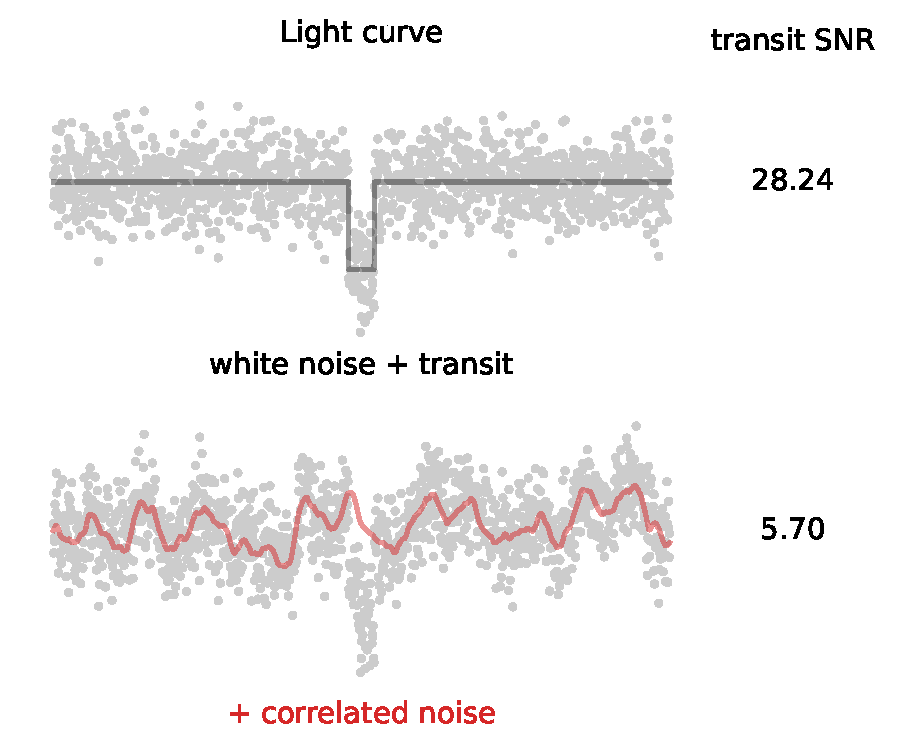
\includegraphics[width=8.5cm]{../figures/issue1.pdf}
        \caption{Illustration of the effect of correlated noise on a single transit signal-to-noise (SNR). A 1-hour transit of depth 1\% is simulated on top of white noise as part of a 24-hours observation with an exposure time of 1 minute (top). Then, in the bottom plot, correlated noise is added to the transit signal and simulated using a Gaussian Process (GP) with a Matèrn-32 kernel of length-scale 1 hour and amplitude 0.2\%. The SNR on the right of each light curve is computed using \autoref{eq:snr}.}
        \label{fig:issue1}
    \end{centering}
\end{figure}

As illustrated in \autoref{fig:issue1}, the presence of correlated noise strongly decreases the transit signal SNR, limiting its detection. This issue rapidly motivated the development of systematics detrending algorithms such as the Trend Filtering Algorithm (\textsc{TFA}, \citealt{tfa}, in its primary use case), \textsc{SysRem} (\citealt{sysrem}), or Pixel Level Decorrelation (\textsc{PLD}, \citealt{pld}; see also \textsc{Everest} from \citealt{everest1, everest2}). Most of these methods rely on the shared nature of instrumental signals among light-curves (or neighboring pixels) such that the correction applied should not degrade the transit signal. We note that, except for \textsc{TFA}, these algorithms are mostly applied to space-based continuous observations, that provide continuous stellar baselines and mostly reproducible systematic signals. This is not the case for the vast majority of ground-based observations, in addition subject to periodic daytime interruptions and varying atmospheric extinction.

\subsection{The effect of detrending on transits detectability}\label{detrending_effect}

Instrumental signals have the benefit to be shared among light curves of stars observed with the same instrument, strongly correlated with measurements from the experimental setup (like detector's temperature, pointing error, sky background or airmass), hence we will make the strong assumption that their detrending based on an incomplete model of the light curve, one that ignore transit signals (because unknowns), do not affect the searched signals. In opposition, stellar variability is generally unknown and harder to correlate with simultaneous measurements. This gave rise to two types of treatments in order to reconstruct and detrend stellar variability, and perform transit search on \textit{flattened} light curves. One is physically-motivated and makes use of Gaussian Processes \citep[e.g.]{k2sc}. The other is empirical and makes use of filtering algorithms (a wide variety being described in \cite{wotan}). In this section, we will study in details the effect of both approaches on transit detectability, by studying the degradation of a unique transit SNR for a wide variety of stellar variability characteristics.
\\\\
Throughout this paper, we simulate stellar variability (and later model it) thanks to Gaussian Processes (GP), employing the physically-motivated stochastically-driven damped simple harmonic oscillator kernel (SHO) presented in \citealt{celerite1}. Extensive details about the following simulations can be found in \autoref{app_principle_simulations}.

\begin{figure}[H]
    \begin{centering}
        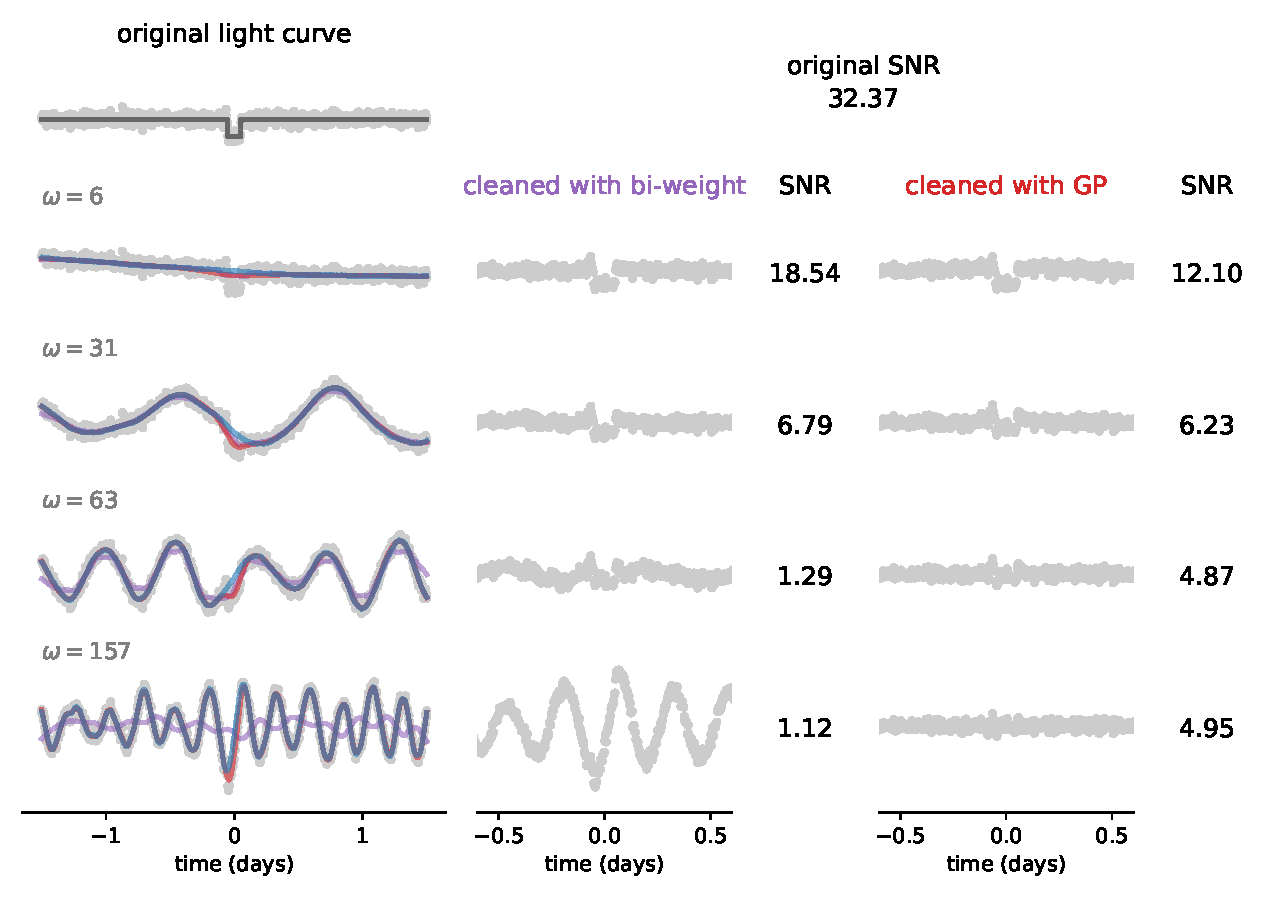
\includegraphics[width=\linewidth]{../figures/issue2.pdf}
        \caption{Simulation of a single non-periodic transit plus various variability signals using the formalism described in \autoref{app_principle_simulations}. For each simulation, the variability is fitted using a biweight filter \citep[in violet]{wotan} and a Gaussian Process (in red, descibed in \autoref{app_gp}, in each case with the same kernel used to generate the data). The fitted variability is then subtracted and the transit SNR computed using \autoref{eq:snr}, with the transit depth estimated as the minimum in-transit flux.}
        \label{fig:issue2}
    \end{centering}
\end{figure}

In \autoref{fig:issue2}, we simulate a light curve featuring a single transit in addition with stellar variability of different timescales and amplitudes. In case \textit{a} (purple in \autoref{fig:issue2}), we model and detrend these signals using the widely-adopted Tukey's biweight filtering method presented in \citealt{tukey} and its implementatation from \texttt{wõtan}\footnote{\href{https://github.com/hippke/wotan}{https://github.com/hippke/wotan}} \citep{wotan}. In case \textit{b} (red in \autoref{fig:issue2}) we employ the same GP model used to simulate stellar variability to reconstruct and remove it from light curves ignoring the presence of potential transits (the case of unknown transits search). Once transits cleaned from stellar variability, we asses their remaining SNR using \autoref{eq:snr}.
\\\\
\autoref{fig:issue2} clearly shows the effect of both detrending techniques on transits SNR, and suggests that this degradation is strongly dependant on the stellar variability characteristics encountered. In order to explore the parameter space for which detrending is the most problematic, we simulate light curves including a single transit and a much wider range of correlated noise characteristics defined with two parameters: $\tau$ the relative timescale of the variability with respect to the transit duration; and $\delta$, the relative amplitude of the variability against transit depth, such that:
\begin{equation}\label{eq:relative_param_space}
    \tau \propto \frac{\mathrm{variability\; timescale}}{\mathrm{transit\;duration}} \quad \text{and} \quad 
    \delta \propto \frac{\mathrm{variability\; amplitude}}{\mathrm{transit\;depth}} 
\end{equation}
To follow this parametrization, we simulate the photometric variability using a GP with an SHO kernel with hyperparameters \footnote{}:
\begin{equation}\label{eq:relative_params}
    \omega = \frac{\pi}{\tau D} \quad 
    \sigma = \delta \frac{\Delta}{2} \quad  \text{and}  \quad  
    Q = 10
\end{equation}
with $\Delta$ and $D$ the depth and duration of the simulated transit, similar in all light curves. 
% We fix a relatively high value for the quality factor $Q$ in order to restrict our simulations to strongly periodic variability signals. 
For $\tau=1$ and $\delta=1$, the expressions of $\omega$ and $\sigma$ given in \autoref{eq:relative_params} correspond to a periodic signal with a period half that of the transit duration, and a peak to peak amplitude two times that of the transit depth, i.e. strongly resembling the simulated transit signal. As in \autoref{fig:issue2}, we reconstruct the variability using a biweight filter with a window length of $3D$ (three times the transit duration, an optimal value according to \citealt{wotan}). We then subtract the variability from each light-curve, estimate the resulting transit depth (using the in-transit minimum flux) and compute its SNR. \autoref{fig:snr_detrend} shows the remaining SNR values of transits computed this way, after each variability signals with random $(\tau, \delta)$ have been detrended.
\\\\
\autoref{fig:snr_detrend} shows that it exists an entire region of the $(\tau, \delta)$ parameter space for which detrending degrades transit SNR to the point of no detection ($SNR < 6$). While this region might only represent a fraction of existing exoplanetary systems, we argue that these systems are of great value for the field of Exoplanetary Science. Indeed, as variability is often linked to the presence of starspots, systems whose  with the stellar photo 


% in is likely to be observed on stars whose equatorial plane lines up with our line of sight, following recent studies on the dynamical evolution of planetary systems \cite{}, hence being most likely to be transited.
\TODO

As a direct consequence, these same starspots are more likely to be occulted by planetary companions, events whose measurement benefits both the study of stellar atmospheres and their concerning impact on planetary atmospheric retrievals \cite{}. Finally, the growing interest of the community for ultra-cool dwarf stars comes with observations done in the infrared, featuring enhanced red noise and variability, leading to lower transit SNR \cite{}. Hence, commonly-used detrending technique (such as the biweight filter studied in this section) make transit-search blind to those pristine systems, motivating the need for a more informed transit search algorithm able to deal with correlated noise. In the next section we present such an algorithm: \texttt{nuance}.

\begin{figure}[H]
    \begin{centering}
        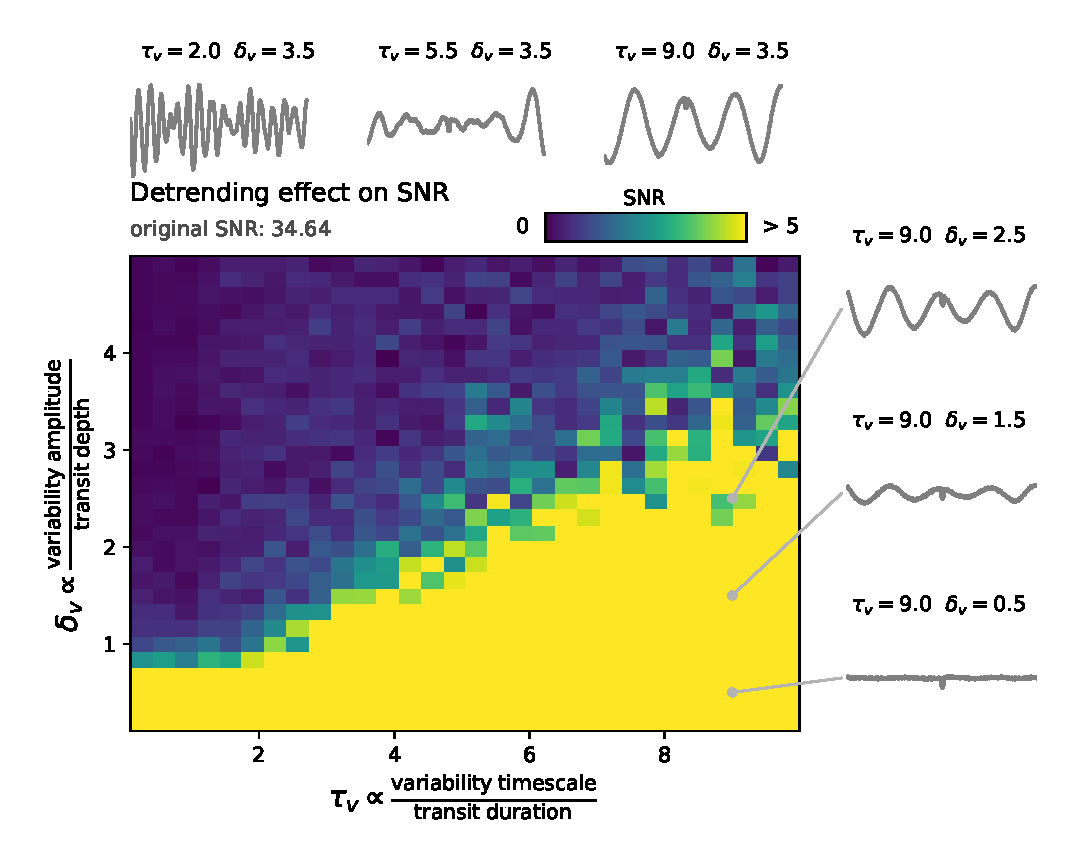
\includegraphics[height=9cm]{../workflows/cleaning_snr/figures/simu1/result.pdf}
        \caption{\TODO{}, and redo plot with top arrows and fix $tau_v$ $delta_v$}
        \label{fig:snr_detrend}
    \end{centering}
\end{figure}

\section{\texttt{nuance}}\label{nuance}

\texttt{nuance} is an algorithm capable of searching for planetary transits in light curves containing correlated noise, such as instrumental signals and stellar photometric variability.
\\\\
Let a flux $f$ of a star measured at time $t$ be sampled and aranged in the $(1\times N)$ column-vector $\bm{f}$. This flux contains instrumental signals, stellar variability and a periodic transit signal that we wish to uncover. An example of such signal is simulated and shown in \autoref{fig:principle_dataset}.

\begin{figure}[H]
    \begin{centering}
        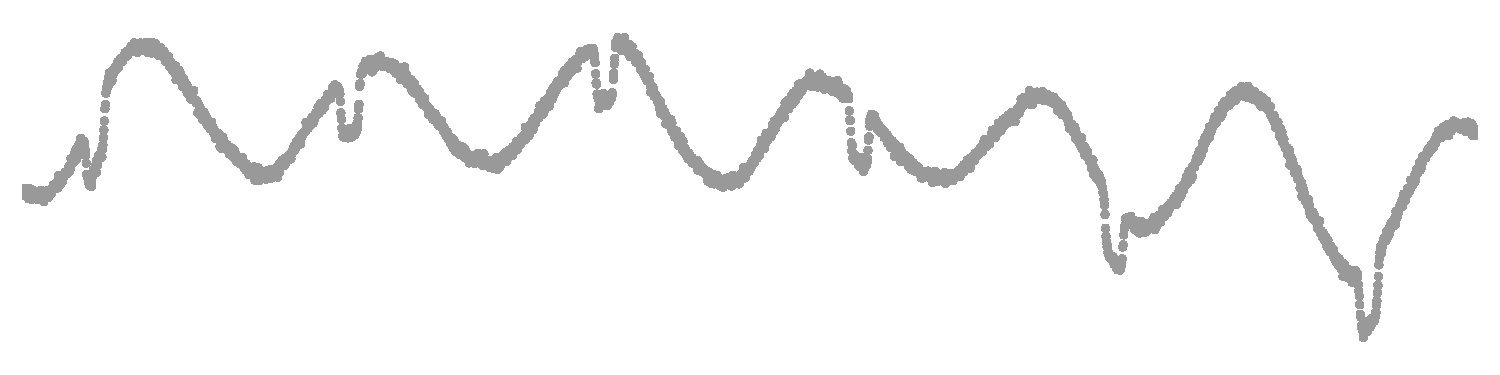
\includegraphics[width=0.7\linewidth]{../figures/principle_dataset.pdf}
        \caption{Simulated light curve containing a periodic transit signal, instrumental systematics, and stellar variability, all described in \autoref{app_principle_simulations}.}
        \label{fig:principle_dataset}
    \end{centering}
\end{figure}

Simultaenously to the flux measurement, we obtained a set of $M$ measurements, aranged in the $(M\times N)$ matrix $\bm{X}$, that can be treated as explanatory variables for $\bm{f}$. Details about the simulation of these signals are provided in \autoref{app_principle_simulations}.
\\\\
Ideally, we would detect such  a periodic transit signal by sampling the posterior likelihood of this data to a full-fledge model including stellar variability (more generally correlated noise), instrumental systematics (modeled with explanatory variables), and a periodic transit signal of period $P$, epoch $T_0$, duration $D$ and depth $\Delta$. We would then reduce the posterior likelihood to $p(\bm{f}\vert P)$, its marginalized version over all parameters except the period $P$, producing a transit search periodogram $\mathcal{Q}(P)$. However, this approach has two issues: It is highly intractable, and it may lead to multimodal distributions that are hard to interpret.
\\\\
Given a period $P$, we instead want to compute the likelihood of a periodic transit signal at the maximum likelihood parameters $\hat T_0$, $\hat D$ and $\hat \Delta$, i.e the periodogram
\begin{equation}\label{eq:periodogram}
        \begin{gathered}
        \mathcal{Q}(P) = p(\bm{f} \vert P, \hat T_0 ,\hat D, \hat \Delta) \\
        \text{where} \quad (\hat T_0 ,\hat D, \hat \Delta) = \argmax_{T_0, D, \Delta}p(\bm{f} \vert P, T_0 , D, \Delta)
    \end{gathered}
\end{equation}
We will do that by adopting the strategy of \cite{foreman2016}, and separate the transit search into two components: the \textit{linear search} and the \textit{periodic search}. During the \textit{linear search}, the likelihood of a single non-periodic transit is computed for a grid of epochs, durations and depths. Then, the \textit{periodic search} consists in combining these likelihoods to compute the likelihood of the data given a periodic transit signal for a range of periods. These combined likelihoods yield a transit-search periodogram on which the periodic transit detection is based. \texttt{nuance} differs by modeling the covariance of the light curve with a Gaussian Process, accounting for correlated noise (especially in the form of stellar variability) while keeping the model linear and tractable.

\subsection{The \textit{linear search}}\label{linear_search}

During the \textit{linear search}, the goal is to compute the likelihood $p(\bm{f} \vert T , D, \Delta)$ of our data given a single non-periodic transit signal of epoch $T$, duration $D$ and depth $\Delta$, for a grid of epochs, durations and depths.
\\\\
To account for correlated noise, we model the light curve $f$ as being drawn from a Gaussian Process such that
$$\bm{f} \sim \mathcal{N}(\bm{w X}, \bm{\Sigma})$$
with mean $\bm{wX}$ (i.e. a linear model of the M explanatory variables with coefficients $\bm{w}$) and covariance $\bm{\Sigma}$. To account for the presence of a single non-periodic transit of epoch $T$ and duration $D$, we compute and append its signal as the last column of the design matrix $\bm{X}$, using the simple transit model from \citealt{protopapas} with a unitary depth (see \autoref{app_proto}). This way, the transit signal is part of the linear model and its depth $\Delta$ can be solved linearly. Under this assumption, the likelihood of the data given a single non-periodic transit is analytical
\begin{equation} \label{eq:linear_search_ll}
    \ln p(\bm{f} \vert I) = -\frac{1}{2}(\bm{f}-\bm{wX})^T\bm{\Sigma}^{-1}(\bm{f}-\bm{wX}) -  \frac{1}{2}\vert\bm{\Sigma}\vert - \frac{N}{2}\ln 2
\end{equation}
and can be computed on a grid of epochs and durations, the transit depth being linearly solved for any $(T, D)$. This \textit{linear search} lead to the set of likelihoods\footnote{This notation omits the vector $\bm{w}_{i,j}$ (except its last value $\Delta_{i,j}$) as it is linearly solved for any given value of $(T_i, F_j)$ and irrelevant in what follows.}
$$\set{\ln\mathcal{L}_{i,j}}_{i, j} = \set{\ln p(\bm{f} \vert T_i ,D_j, \Delta_{i,j})}_{i, j}$$
were $\Delta_{i,j}$ is the depth linearly solved for a given $(T_i, D_j)$. \autoref{fig:linear_search} shows this likelihood grid computed for the simulated dataset shown in \autoref{fig:principle_dataset}, using the same Gaussian Process and design matrix $\bm{X}$ used to simulate the data (see \autoref{app_gp}).

\begin{figure}[H]
    \begin{centering}
        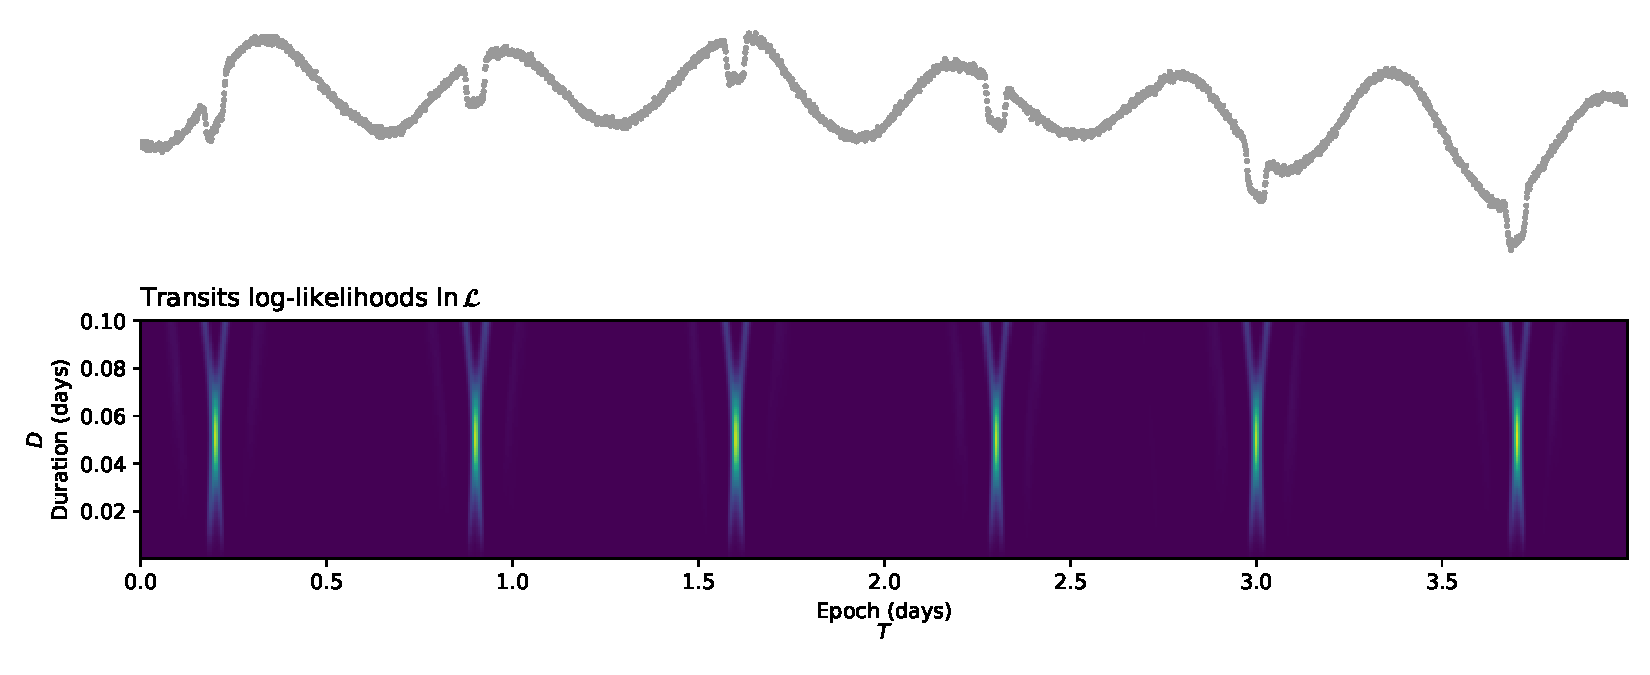
\includegraphics[width=0.95\linewidth]{../figures/principle_linear_search.pdf}
        \caption{Principle and output of the \textit{linear search}. First, a set of durations and depths $\set{T_i, D_j}_{i,j}$ is generated. For each pair of index $(i,j)$, the likelihood $\ln p(\bm{f} \vert T_i ,D_j, \Delta_{i,j})$ is computed, using the parameters from \autoref{eq:ls} and the expression of \autoref{eq:linear_search_ll}. This process yields the grid of likelihoods $\ln\mathcal{L}$ (bottom plot), as well as the $\set{\Delta_{i,j}, \sigma_{i,j}}_{i, j}$ transit depths and errors inferred linearly.}
        \label{fig:linear_search}
    \end{centering}
\end{figure}

To prepare the next step, the corresponding depths $\Delta_{i,j}$ linearly solved for any $(T_i ,D_j)$ are conserved, as well as their associated errors $\sigma_{i,j}$ obtained through the least-square solution
\begin{equation}\label{eq:ls}
    \begin{gathered}
        \bm{w} = (\bm{X}^T\bm{\Sigma}^{-1}\bm{X})^{-1}\bm{X}^T\bm{\Sigma}^{-1}\bm{f} \\
        \bm{\sigma} = (\bm{X}^T\bm{\Sigma}^{-1}\bm{X})^{-1}
    \end{gathered}
\end{equation}    
where $\Delta_{i,j} = \bm{w}_M$ and $\sigma_{i,j} = \bm{\sigma}_{MM}$

\subsection{The periodic search}

We then need to combine the likelihoods computed from the \textit{linear search} to obtain
\begin{equation}\label{eq:goal}
    p(\bm{f} \vert P, T_0 , D, \Delta)
\end{equation}
For a given transit duration $D$, any combination of $(P, T_0)$ leads to K truly independent transits, for which it is tempting to write
\begin{equation}\label{eq:attempt}
    p(\bm{f} \vert P, T_0 ,D, \Delta) = \prod_k^K p(\bm{f} \vert T_k, D, \Delta_k)
\end{equation}
where $\set{T_k}_k$ are the epochs matching $(T_0, P)$ and $\set{\Delta_k}_k$ the corresponding depths. So that
$$
    \ln p(\bm{f} \vert P, T_0 ,D, \Delta) = \sum_k^K \ln \mathcal{L}_k
$$
This is the joint likelihood of transits belonging to the same periodic signal but with varying depths  $\set{\Delta_k}_k$. However, individual transits from a periodic signal cannot be considered independent, and should instead share a common transit depth $\Delta$. We show in \autoref{combining_transits} that there is an analytical expression for the joint likelihood of K individual transits with depths and errors $\set{\Delta_k, \sigma_k}_k$ assuming a common depth $\Delta$:
\begin{equation}\label{eq:comb}
    \begin{gathered}
        \ln p(\bm{f} \vert P, T_0 ,D, \Delta) =  \sum_{k}^K \ln \mathcal{L}_k  - \frac{1}{2} \sum_k^K\left(\ln(\sigma_{k}^2) - \ln(\sigma^{2} + \sigma_{k}^{2}) +  \frac{\left(\Delta_{k} -
        \Delta\right)^{2}}{\sigma_k^{2} + \sigma^{2}}\right) \\
        \text{with} \quad  \frac{1}{\sigma^2} = \sum_k^K \frac{1}{\sigma_k^2} \quad \text{and} \quad
        \Delta = \sigma^2 \sum_k^K {\frac{\Delta_k}{\sigma_k^2}}
    \end{gathered}
\end{equation}

While this gives a solution for \autoref{eq:goal}, the individual epochs matching $T_0$ and $P$ are not necessarily available in the grid of epochs $\set{T_k}_k$. In \cite{foreman2016} a similar issue is solved by using the nearest neighbors in the epochs grid. Instead, to allow the efficient matrix computation of \autoref{eq:comb}, we interpolate the likelihood grid from $\set{T_i}_i$ to a common grid of transit phases $\set{\phi_i}_i$, leading to the \textit{periodic search} log-likelihood
$$\ln\mathcal{P}(P) = \set{\ln p(\bm{f} \vert P, \phi, D)}_{i,j}$$
shown for few periods in \autoref{fig:periodic_search}.b. In the latter equation, $\Delta_{i,j}$ is omitted since being interpolated from the \textit{linear search} using $\phi_i$, $D_j$ and $T_0 = 0$.

\begin{figure}[H]
    \begin{centering}
        \gridline{\fig{../figures/principle_periodic_0.pdf}{0.95\linewidth}{\vspace{-0.5cm}(a) $\ln \mathcal{L}$}}
        \vspace{-0.6cm}
        \gridline{\fig{../figures/principle_periodic_1.pdf}{0.72\linewidth}{\vspace{-0.5cm}(b) $\mathcal{P}(P)$}}
        \caption{On the example dataset, this figure shows how the \textit{periodic search} works at different periods $P$ (including the true period $P = 0.7$ days). Given $P$ and $T_0=0$, the likelihood $\ln\mathcal{L}$ shown in (a) is phase-folded and interpolated onto a common grid of phases shown in (b). As an example, the white lines in (a) mark the edges of each fold for a period of $P=0.5$ days, and the white crosses show the epochs $\set{T_k}_{k\in\mathbb{K}}$ matching a particular phase in the grid (reported in (a) and (b)) on which the corresponding $\set{\ln \mathcal{L}_k}_{k\in\mathbb{K}}$ are interpolated and combined using \autoref{eq:comb}. To allow the use of efficient matrix computations, this is done for all durations $\set{D_i}_i$ so that $\mathcal{P}$ is computed on the full grid $\set{D_i, \phi_i}_{i, j}$ at once. We understand from the folded likelihoods plots in (b) that a different choice of epoch $T_0$ may only shift the results in phase but do not affect the values of $\mathcal{P}$. For this reason, computing $\mathcal{P}$ for $T_0=0$ is sufficient. We also notice how the maximum value of $\mathcal{P}(P=0.7/2)$ is lower than for $P=0.7$ days, a result of combining the log-likelihoods using \autoref{eq:comb} instead of \autoref{eq:attempt}, in favor of individual transits matching a common depth $\Delta$.}
        \label{fig:periodic_search}
    \end{centering}
\end{figure}



\subsection{The transit search periodogram}

Using \autoref{eq:comb}, we can now compute $\ln\mathcal{P}$ for a range of periods and build a transit search periodogram using \autoref{eq:periodogram}. But a final issue emerges, one that is fundamentally linked to our strategy. Each likelihood $p(\bm{f} \vert T, D, \Delta)$ estimated during the \textit{linear search} is computed using N measurements. Hence, combining transits in the \textit{periodic search}, through $\Delta_k$, $\sigma_k$ and the product of $K$ likelihoods $\set{\mathcal{L}_k}_k$ (\autoref{eq:comb}), artificially leads to a likelihood involving $N\times K$ measurements. This lead to a normalization issue when trying to compare the joint log-likelihoods $\mathcal{P}(P)$ from one period to another (like the ones in \autoref{fig:periodic_search} that have been normalized for visualization purpose), as the number of observed transits differs from one period to another. This motivates a final step to produce the transit search periodogram $Q$. For any period P, instead of taking $ \mathcal{Q}(P)$ as the maximum value of $\ln\mathcal{P}$, we retrieve the maximum likekihood parameters
\begin{equation}\label{eq:phi0}
    (\phi_0 ,D) = \argmax_{\phi_i, D_j} \set{\ln p(\bm{f} \vert P, \phi_i, D_j)}_{i, j}
\end{equation}
and define $\mathcal{Q}(P)$ as the SNR of the transit of period $P$, epoch $T_0 = \phi_0 P$, duration $D$ and depth $\Delta$, i.e.
$$
    \mathcal{Q}(P) = \frac{\Delta}{\sigma}
$$
where $\Delta$ and $\sigma$ are obtained using \autoref{eq:comb} with the last column of $X$ containing a periodic transit signal of period $P$, epoch $T_0$, duration $D$ and depth $1$. This process and the resulting periodogram $\mathcal{Q}$ are shown in \autoref{fig:periodogram}.

\begin{figure}[H]
    \begin{centering}
        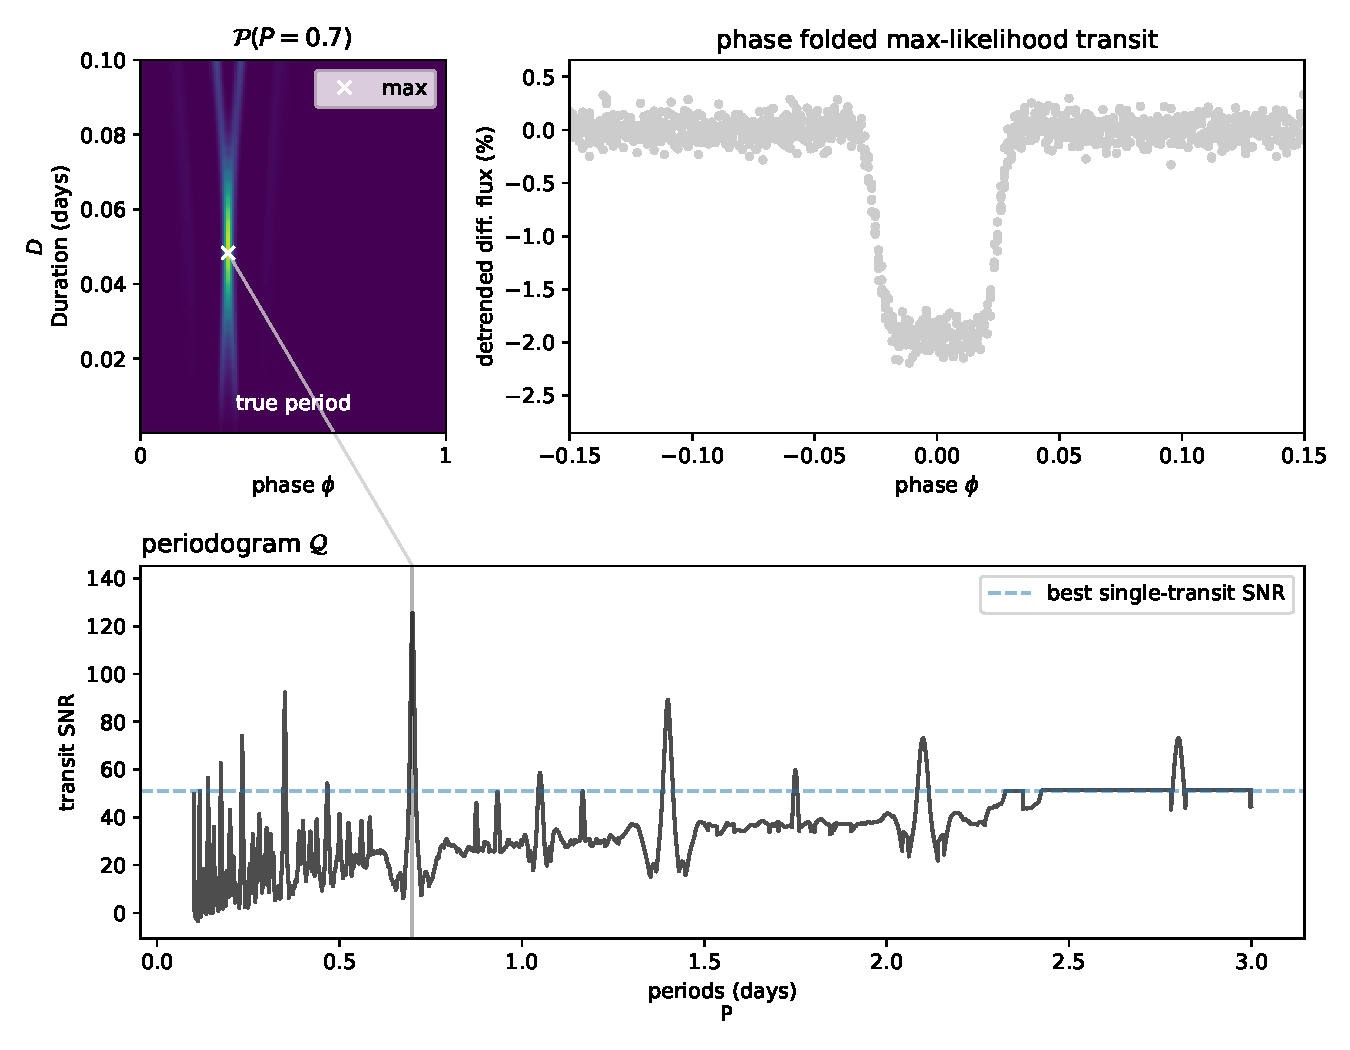
\includegraphics[width=0.8\linewidth]{../figures/principle_Q.pdf}
        \caption{For each period $P$, the joint likelihood $\mathcal{P}(P)$ of matching transits is computed using \autoref{eq:comb}, and the value of the maximum likelihood transit SNR retained as $\mathcal{Q}(P)$.}
        \label{fig:periodogram}
    \end{centering}
\end{figure}

The periodic transit of period $P$ with the maximum SNR, i.e. maximizing $\mathcal{Q}$, is adopted as the best candidate, basing our confidence in this signal through its SNR. The parameters of this transit are the period $P$, the epoch $T_0 = \phi_0 P$ and duration $D$ (\autoref{eq:phi0}), and the depth $\Delta$ with error $\sigma$ (\autoref{eq:comb}).

\newpage
\subsection{An open-source python package}
We implement the methods described in this paper in the open-source Python package \nuance{}, hosted on Github\footnote{\href{https://github.com/lgrcia/nuance}{https://github.com/lgrcia/nuance}} with an extensive user documentation\footnote{\href{https://nuance.readthedocs.io}{https://nuance.readthedocs.io}}.
\\\\
To instantiate a search, a user can start by creating a \texttt{Nuance} object with
\begin{lstlisting}[language=Python]
    from nuance import Nuance

    nu = Nuance(time, flux, error, kernel, X)
\end{lstlisting}
where \texttt{kernel} is the kernel of the Gaussian Process used to model corelated noise, and \texttt{X} the design matrix of the linear model. \nuance{} exploits the Gaussian Process implementation from \texttt{tinygp}\footnote{\href{https://github.com/dfm/tinygp}{https://github.com/dfm/tinygp}}, a Python package powered by \texttt{JAX}\footnote{\href{https://github.com/google/jax}{https://github.com/google/jax}} allowing for custom kernels to be built and highly tractable computations. We can then define a set of epochs \texttt{t0} and durations \texttt{Ds} and run the \textit{linear search} with
\begin{lstlisting}[language=Python]
    import numpy as np

    t0s = time.copy()
    # a range of 20 durations
    Ds = np.linspace(0.01, 0.2, 10)
    nu.linear_search(t0s, Ds)
\end{lstlisting}
Finally, the \textit{periodic search} is run with
\begin{lstlisting}[language=Python]
    # a wide range of periods
    periods = np.linspace(0.1, 5, 2000)
    search = nu.periodic_search(periods)
\end{lstlisting}
From this \texttt{search} object, the best transiting candidate parameters can be computed (\texttt{search.best}), or the $\mathcal{Q}$ periodogram retrieved (\texttt{search.Q\_snr}), together with valuable information about the transit search. The \texttt{Nuance} object also provides methods to perform transit search on light curves from multi-planetary systems, the advantage of \texttt{nuance} being that the \textit{linear search} only needs to be performed ones, and reused for the search of several transiting candidates. An extensive and maintained online documentation is provided at \href{https://nuance.readthedocs.io}{\texttt{nuance.readthedocs.io}}.

\newpage
\section{Validation with injection-recovery}\label{simu}
In order to validate our algorithm, we assess the transit search capabilities of \texttt{nuance} against commonly used techniques. As demonstrated in \autoref{detrending_effect}, the full-fledged modeling offered by \texttt{nuance} is not always necessary, and becomes beneficial for particular noise characteristics that are relative to the searched transit parameters. Hence, our comparison will be done on the relative parameter space $(\tau, \delta)$ described in \autoref{eq:relative_param_space}, focusing on its formulation by assuming correlated noise in the form of stellar variability (\autoref{eq:relative_params}) simulated using a Gaussian Process with an SHO kernel (\autoref{app_gp}). Ultimately, we demonstrate in this section how \texttt{nuance} compares with commonly used techniques, depending on the similarity between stellar variability and the searched transit signals.
\\\\
In what follows, we inject transits in simulated or real datasets, and employ algorithms to recover these transits with the right parameters (hence \textit{injection-recovery}). We consider the transit to be found if the absolute difference between the periods $dP$ and epochs $dT_0$ of the recovered and injected planets follow
$$dP<0.1\;\text{days} \hspace{0.5cm} \text{and} \hspace{0.5cm} dT_0<0.01\;\text{days}$$ 

\newcommand{\wtls}{\texttt{wõtan+TLS}}

\subsection{Comparison with \wtls{} on a simulated light curves}

We start by comparing \texttt{naunce} to a relatively simple method on simulated light curves. As in \autoref{detrending_effect}, this simple method consist in searching for planetary transits by first modeling stellar variability using an optimal biweight filter (implemented in \texttt{wõtan} \citep{wotan} using a window size three times that of the injected transit duration), subtracting it from the light-curve, and then perform the search on the detrended light curve using an optimal box-least-square algorithm (\texttt{TLS}, \citealt{tls}). We name this method \wtls{}.
\\\\
The dataset consists in 10 000 light curves simulated using the model described in \autoref{app_principle_simulations}. We simulate a common periodic transit among all light curves, of period $P=1.1$ days, epoch $T_0=0.2$ days, duration $D=0.04$ days and depth $\Delta=2\%$. Each light curve consist in a 3 days observation, with an exposure time of 2 minutes, leading to $N=2160$ data points with a normal error of $0.1\%$.
\\\\
For a given pair of $(\tau, \delta)$, we simulate stellar variability using a Gaussian Process with an SHO kernel of hyperparameters defined by \autoref{eq:relative_params}, computed with respect to the injected transit parameters $D$ and $\Delta$. The same kernel is used for the search with \texttt{nuance}, an optimal choice on equal footing with the optimal biweight filter employed in the \wtls{} search. We generate 10 000 pairs of $(\tau, \delta)$ such that
$$\tau \sim \mathcal{U}(0.1, 40)\hspace{0.5cm}\text{and}\hspace{0.5cm} \delta \sim \mathcal{U}(0.1, 100)$$
where $\mathcal{U}(a, b)$ denotes a uniform distribution of lower bound $a$ and upper bound $b$.
\\\\
The results of these injection-recovery are shown in \autoref{fig:simu} and highlight particularly well the benefit of \nuance{} against \wtls{} on transits corresponding to $\delta > 3$ and $\tau > 2$, i.e. with relatively low transit depth compared to the stellar variability amplitude, and a relatively small duration compared to the stellar variability period. On average, searching a single light curve with \nuance{} took 9 seconds, compared to 8 seconds with \wtls{}. Beyond its increased sensitivity, this metric demonstrates the tractability of \nuance{}, studied in more details in \autoref{}.
\\\\
About these results, we note these transit searches were done in a particularly optimal setup, on light curves not all physically realistic, hence demonstrating the performance of \nuance{} on a theoretical basis only. In the next subsection, we perform transits injection-recovery on a real dataset, using more realistic tools and on light curves featuring known planetary transits, hence validating \nuance{} on a realistic multi-planetary dataset.


\begin{figure}[H]
    \begin{centering}
        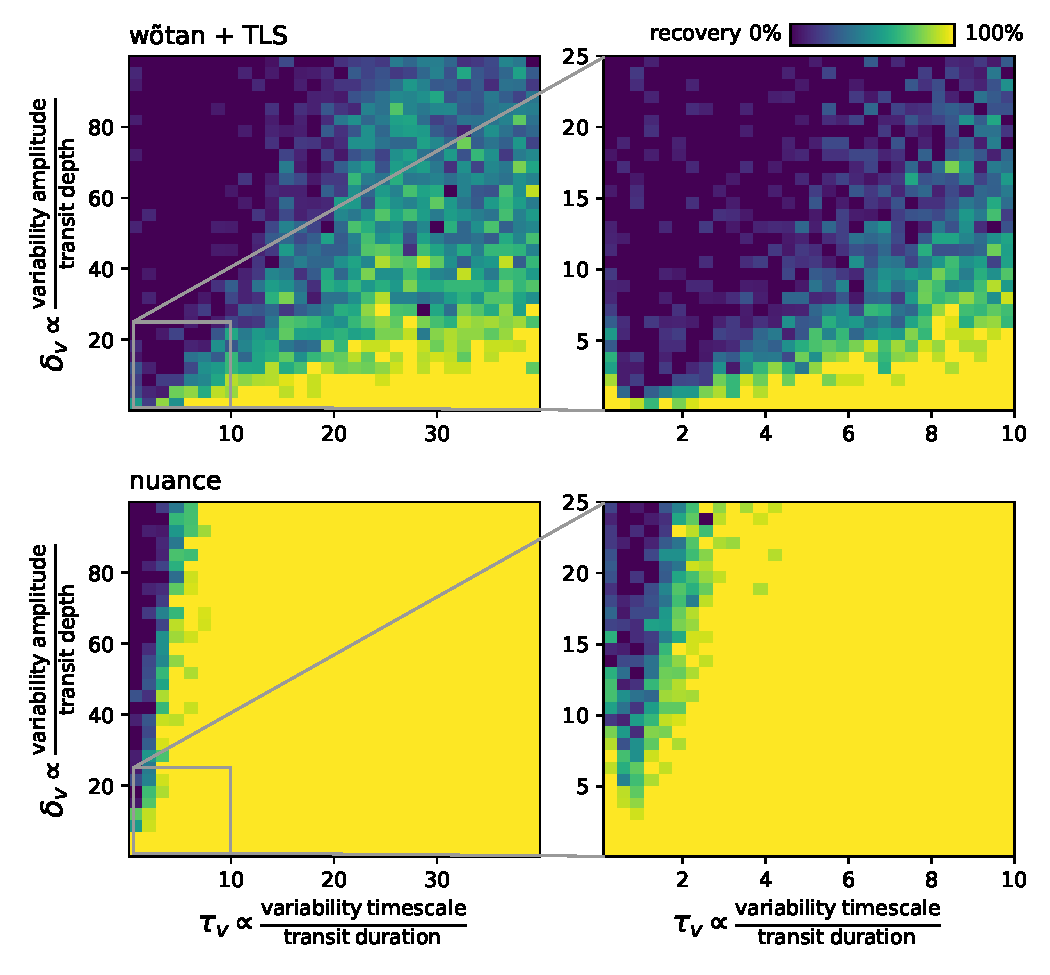
\includegraphics[height=12cm]{../workflows/synthetic_injection_recovery/figures/final_result.pdf}
        \caption{\TODO}
        \label{fig:simu}
    \end{centering}
\end{figure}

\subsection{Comparison with \texttt{Sherlock} on TOI-540 real light curves}\label{real}

\section{Performances and limitations}\label{perf}
\TODO

\section{Conclusion}
\TODO
\\\\
We would like to thank Julien De Wit and Prajwal Niraula for meaningful discussions at the begining of the project, Germain Garcia for his useful insights about numerical optimization, and Michaël Gillon for his overall support. Co-author Daniel Foreman-Mackey helped in shaping the mathematical formalism of our method and introduced the use of \texttt{JAX} for its tractable implementation. Co-author Francisco J. Pozuelos was key in validating \texttt{nuance} on real datasets.

\newpage
\appendix
\section{Light curve simulations}\label{app_principle_simulations}

\definecolor{blue_S}{rgb}{0.12156862745098039, 0.4666666666666667, 0.7058823529411765}
\definecolor{red_V}{rgb}{0.8392156862745098, 0.15294117647058825, 0.1568627450980392}

% This paper relies on simulated light curves featuring periodic transit signals, instrumental signals and correlated noises such as stellar variability. To do so, we draw $\bm{f}$ from a Gaussian Process of mean $\bm{\mu}$ with $\mu_i = {\color{Gray}{\mathcal{T}}}(t_i) + {\color{blue_S}{\mathcal{S}}}(t_i)$, where and covariance matrix $\bm{C}$ with $C_{i, j} = {\color{red_V}\nu}(t_i, t_j)$ 

Let $f$ be the simulated flux of a star sampled and aranged in the $(1\times N)$ column-vector $\bm{f}$ associated to the column-vector of times $\bm{t}$. We construct $\bm{f}$ such that
$$
    \bm{f} \sim \mathcal{N}(\bm{\mu}, \bm{C})
$$
The mean $\bm{\mu}$ is built such that $\mu_i = \mathcal{T}(t_i) + \mathcal{S}(t_i)$ where $\mathcal{T}$ is a periodic transit signal and $\mathcal{S}$ an instrumental signal. The covariance matrix $\bm{C}$ is built such that $C_{i, j} = \nu(t_i, t_j)$ where $\nu$ is a covariance function accounting for correlated noise in the form of stellar variabilty with added white noise. An example of such signal is simulated and shown in \autoref{fig:app_principle_dataset}.

\begin{figure}[H]
    \begin{centering}
        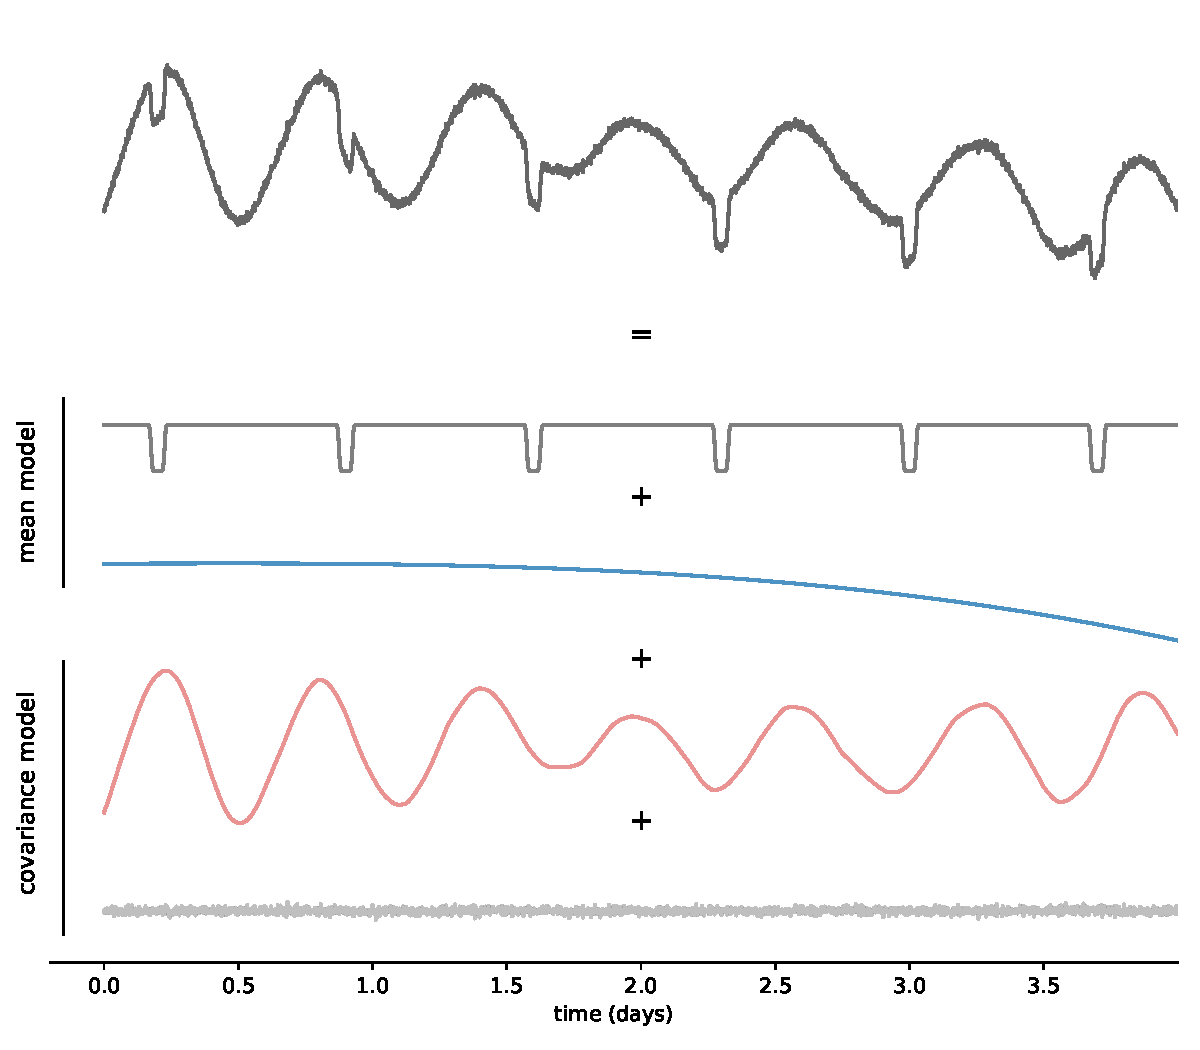
\includegraphics[width=0.8\linewidth]{../figures/principle_dataset_decomposed.pdf}
        \caption{Example dataset sampled at $N=2880$ times corresponding to an observation of 4 days with an exposure time of 2 minutes. The mean of this signal consists in a periodic transit signal plus instrumental signals. Stellar variability and white noise are simulated by modeling the covariance matrix of the signal with Gaussian Processes .}
        \label{fig:app_principle_dataset}
    \end{centering}
\end{figure}
In what follows, we describe the models used to simulate the components of the signal $f$, i.e. the periodic transit $\mathcal{T}$, the instrumental systematics $\mathcal{S}$ and the covariance function $\nu$ describing stellar variability and white noise.

\subsection{Transit signal $\mathcal{T}$}\label{app_proto}
We simulate the periodic transit signal $\mathcal{T}$ using the simple model described in \cite{protopapas} where a transit of period $P$, epoch $T_0$, duration $D$ and unitary depth observed at time $t$ is given by
\begin{equation}
    \begin{gathered}
        \mathcal{T}_c(t, P, T_0, D) = \frac{1}{2}\tanh\left(c\left(\theta - \frac{1}{2}\right)\right) - \frac{1}{2}\tanh\left(c\left(\theta + \frac{1}{2}\right)\right) \\
        \text{with}\quad\theta = \frac{P}{\pi  D}\sin\left(\frac{\pi(t-T_0)}{P}\right)
    \end{gathered}
\end{equation}
where the dimensionless parameter c controls the roundness of the transit depth ($c\gg1$ corresponding to a box-shaped transit as shown in \autoref{fig:protopapas}). This analytical model is fully empirical but easily differentiable. From this expression, we get the signal of the single non-periodic transit of unitary depth 
\begin{proof}{single_transits}\label{eq:protopapas_single}
    \tau_c(t, T_0, D) = \lim_{P\to \infty} \mathcal{T}(t, P, T_0, D) = -\frac{1}{2}\tan\left(\frac{c}{2}(1-T_0+t)\right) -\frac{1}{2}\tan\left(\frac{c}{2}(1+T_0-t)\right)
\end{proof}
with epoch $T_0$ and duration $D$.

\begin{figure}[H]
    \begin{centering}
        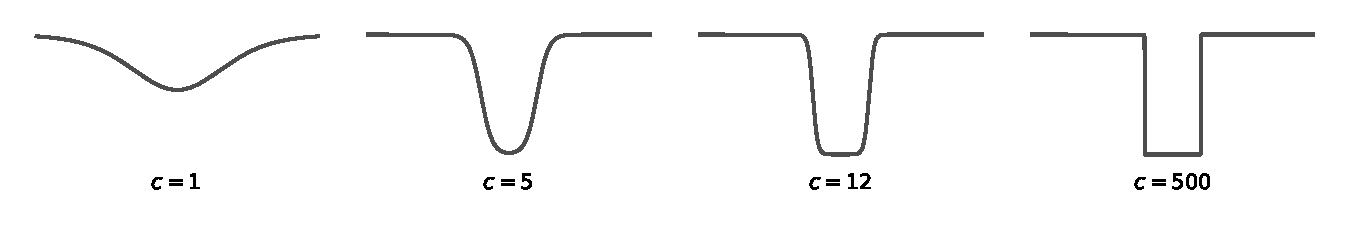
\includegraphics[width=0.9\linewidth]{../figures/protopapas.pdf}
        \caption{Simulations of the single non-periodic transit signal $\tau_c(t, T_0, D)$ (\autoref{eq:protopapas_single}) for different values of $c$}
        \label{fig:protopapas}
    \end{centering}
\end{figure}
In our study, we simulate all transit signals with $c=12$. The periodic transit signal $\mathcal{T}$ seen in \autoref{fig:app_principle_dataset} corresponds to $\mathcal{T} = \mathcal{T}_{c=12}(\bm{t}, P=0.7, T_0=0.2, D=0.05)$, all parameters in unit of \textit{days}.

\subsection{Instrumental signals $\mathcal{S}$}
We simulate instrumental signals as a linear model of $M$ explanatory variables arranged in the $(M\times N)$ design matrix $\bm{X}$. Hence,
$$
    \mathcal{S} = \bm{w}\bm{X}
$$
where the vector $\bm{w}$ are linear coefficients of the model. The simulated flux shown in \autoref{fig:app_principle_dataset} contains a linear model where the $M=4$ columns of the design matrix $\bm{X}$ are given by $\bm{X}_{i} = \bm{t}^i$ (i.e. $\bm{X}$ is the Vandermonde matrix order $3$ of time $t$) and $\bm{w} = [1.0\quad0.0005\quad\text{-}0.0002\quad\text{-}0.0005].$

\subsection{Stellar variability $\nu$}\label{app_gp}
We simulate correlated noise thanks to Gaussian Processes. In our study, we are particularly interested in stellar variability and its effect on transit detection. For this reason, we use a physically-motivated kernel, describing the covariance of a stochastically-driven damped harmonic oscillator (SHO, \cite{, celerite, celerite2}) taking the form 

\begin{equation}
    \begin{gathered}
        k(\tau) = \sigma^2\,\exp\left(-\frac{\omega\,\tau}{2\,Q}\right)
        \left\{\begin{array}{ll}
            1 + \omega\,\tau & \mbox{for } Q = 1/2 \\
            \cosh(f\,\omega\,\tau/2\,Q) + \sinh(f\,\omega\,\tau/2\,Q)/f
                & \mbox{for } Q < 1/2 \\
            \cos(g\,\omega\,\tau/2\,Q) + \sin(g\,\omega\,\tau/2\,Q)/g
                & \mbox{for } Q > 1/2
        \end{array}\right. \\
        \text{where}\quad \tau = |t_i - t_j|\text{,}\quad f = \sqrt{1 - 4\,Q^2} \quad \text{and}\quad g = \sqrt{4\,Q^2 - 1}
    \end{gathered}
\end{equation}
We use this kernel through its implementation in the \texttt{tinygp}\footnote{\href{https://github.com/dfm/tinygp}{https://github.com/dfm/tinygp}} Python package, providing an implententation of the quasi-separable kernel from \citealt{celerite2} powered by \texttt{JAX}\footnote{\href{https://github.com/google/jax}{https://github.com/google/jax}}. The stellar variability signal in \autoref{fig:app_principle_dataset} has been sampled from a Gaussian Process with an SHO kernel of parameters $\omega = \pi/6D$ (i.e. a period equal to 12 times the duration $D$ of the simulated transit), $Q=45$ and $\sigma=\Delta$, the depth of the simulated transit. An extra term $\sigma_f^2=0.001^2$ is added to the covariance matrix, corresponding to the variance of the simulated measurement $f$ and leading to the white noise observed in \autoref{fig:app_principle_dataset}.

\newpage
\section{Combining transits}\label{combining_transits}

\newcommand{\sumTk}{i\neq k}
From the \textit{linear search}, we retain and index by $k$ the parameters of the $K$ individual transits whose epochs $\{T_k\}_k$ are compatible with a periodic signal of period $P$ and epoch $T_0$. From the likelihoods of these transits (computed in \autoref{linear_search}), we want an expression for
\begin{equation}\label{eq:goal2}
    p(\bm{f} \vert P, T_0 ,D, \Delta) = \prod_{k\in\mathbb{T}} p(\bm{f} \vert T_k, D, \Delta)
\end{equation}

i.e., given a depth $D$, the likelihood of our data given a periodic transit signal of period $P$, epoch $T_0$ and a common depth $\Delta$. Since only $\{p(\bm{f} \vert T_k, D, \Delta_k)\}_{k}$ is known (i.e. transits with different depths), we decompose
\begin{equation}\label{eq:non_part_of_per}
    p(\bm{f} \vert T_k, D, \Delta) = \int p(\bm{f} \vert T_k, D, \tilde\Delta)p(\tilde\Delta | \Delta)\, d\tilde\Delta
\end{equation}
where $p(\bm{f} \vert T_k, D, \tilde\Delta)$ is the probability of the $k$-th transit to have a depth $\tilde\Delta$ and $p(\tilde\Delta | \Delta)$ the probability to observe the depth $\tilde\Delta$ knowing the existence of a common depth $\Delta$. In other words, \autoref{eq:non_part_of_per} involves the likelihood of the non-periodic transit $k$ to be part of a periodic transit signal with a common depth $\Delta$.
\\\\
Since each depth $\Delta_k$ is found through generalized least square, each follow a normal distribution $\mathcal{N}(\Delta_k, \sigma_k^2)$, centered on $\Delta_k$ with variance $\sigma_k^2$, and with an amplitude $\mathcal{L}_k$, leading to the likelihood function:
$$p(\bm{f} \vert T_k, D, \tilde\Delta) = \mathcal{L}_k\exp \left(-\frac{(\tilde\Delta-\Delta_k)^2}{2\sigma_k^2}\right)$$
\\\\
As for the common transit depth $\Delta$, it can be estimated through the joint probability of all other transit depths than $\Delta_k$, such that
$$\Delta \sim \prod_{\sumTk}^K \mathcal{N}(\Delta_i, \sigma_i^2)$$
with 
\begin{equation}\label{eq:params}
\frac{1}{\sigma^2} = \sum_{\sumTk}^K \frac{1}{\sigma_i^2} \hspace{0.5cm} \text{and} \hspace{0.5cm}
\Delta =\sigma^2 \sum_{\sumTk}^K {\frac{\Delta_i}{\sigma_i^2}}
\end{equation}
Hence
$$p(\tilde\Delta | \Delta) = \frac{1}{\sqrt{2\pi\sigma^2}}\exp \left(-\frac{(\tilde\Delta-\Delta)^2}{2\sigma^2}\right)$$
We can now rewrite \autoref{eq:non_part_of_per} as
\begin{equation}\label{eq:ice_int}
    p(\bm{f} \vert T_k, D, \Delta) =  \frac{\mathcal{L}_k}{\sqrt{2\pi\sigma^2}} \int \exp\left(-\frac{(\tilde\Delta-\Delta_k)^2}{2\sigma_k^2}\right)\, \exp\left(-\frac{(\tilde\Delta-\Delta)^2}{2\sigma^2}\right)\, d\tilde\Delta
\end{equation}
The integral in \autoref{eq:ice_int} is a product of gaussian integrals that can be obtained analytically and we have
\begin{proof}{gaussians_product_integral}
    p(\bm{f} \vert T_k, D, \Delta) = \mathcal{L}_k  \sqrt{\frac{\sigma_{k}^2}{\sigma^{2} + \sigma_{k}^{2}}} \exp\left(-\frac{1}{2}\frac{(\Delta_k-\Delta)^2}{\sigma_k^2 + \sigma^2}\right)
\end{proof}
And \autoref{eq:goal} gives 
\begin{equation}\label{eq:result}
    \ln p(\bm{f} \vert P, T_0 ,D, \Delta) =  \sum_{k}^K \ln \mathcal{L}_k  - \frac{1}{2} \sum_k^K\left(\ln(\sigma_{k}^2) - \ln(\sigma^{2} + \sigma_{k}^{2}) +  \frac{\left(\Delta_{k} -
    \Delta\right)^{2}}{\sigma_k^{2} + \sigma^{2}}\right)
\end{equation}
the log-likelihood of our data given a periodic transit signal of period $P$, epoch $T_0$, duration $D$ and common depth $\Delta$. In order to reduce the number of times \autoref{eq:params} is computed, we adopt the biased estimates
$$\frac{1}{\sigma^2} = \sum_{k}^K \frac{1}{\sigma_i^2} \hspace{0.5cm}\text{and}\hspace{0.5cm} \Delta  = \sigma^2 \sum_{k}^K {\frac{\Delta_i}{\sigma_i^2}}$$
so that $\Delta$ and $\sigma$ are independent of $k$ in the last sum of \autoref{eq:result}.

\bibliography{bib}

\end{document}
